% Created by tikzDevice version 0.8.1 on 2015-06-10 21:23:12
% !TEX encoding = UTF-8 Unicode
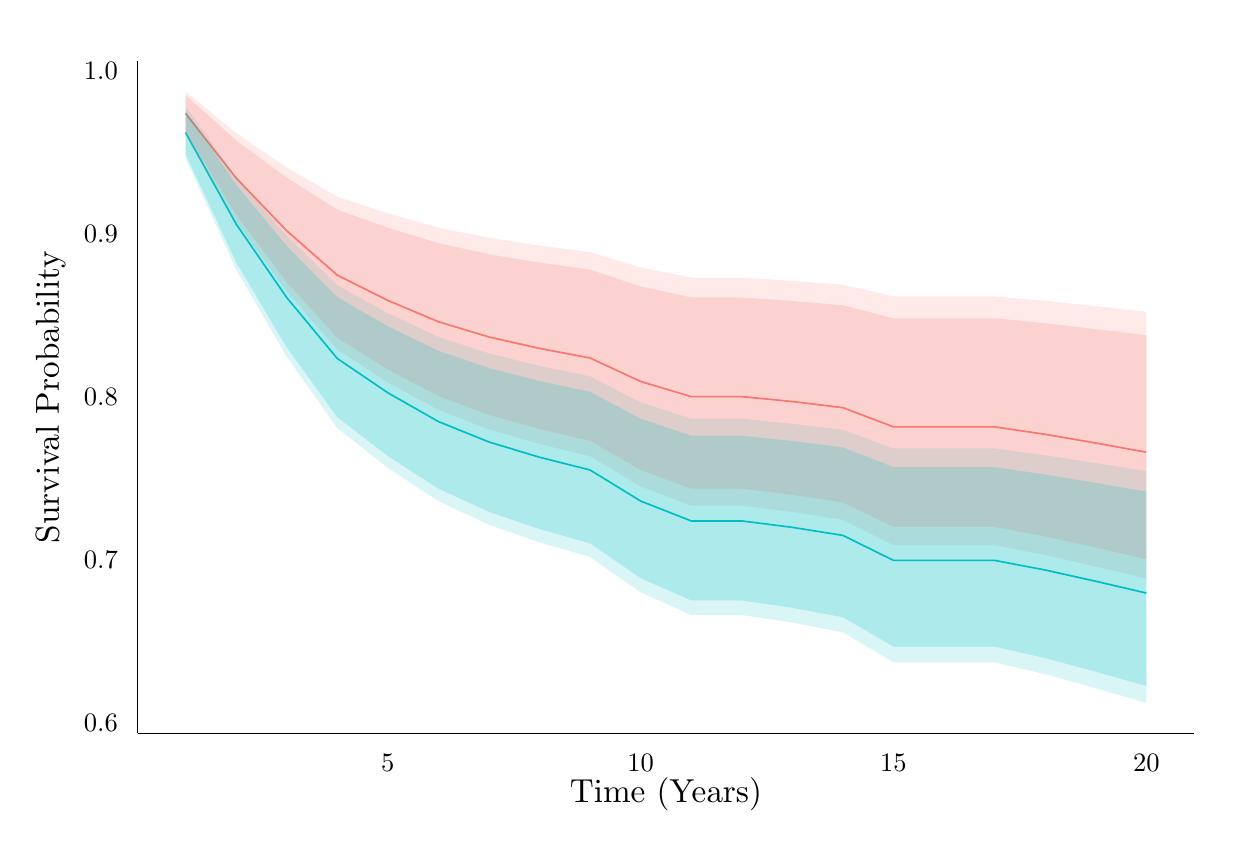
\begin{tikzpicture}[x=1pt,y=1pt]
\definecolor{fillColor}{RGB}{255,255,255}
\path[use as bounding box,fill=fillColor,fill opacity=0.00] (0,0) rectangle (433.62,289.08);
\begin{scope}
\path[clip] (  0.00,  0.00) rectangle (433.62,289.08);
\definecolor{drawColor}{RGB}{255,255,255}
\definecolor{fillColor}{RGB}{255,255,255}

\path[draw=drawColor,line width= 0.6pt,line join=round,line cap=round,fill=fillColor] (  0.00,  0.00) rectangle (433.62,289.08);
\end{scope}
\begin{scope}
\path[clip] ( 39.69, 34.03) rectangle (421.57,277.03);
\definecolor{fillColor}{RGB}{255,255,255}

\path[fill=fillColor] ( 39.69, 34.03) rectangle (421.58,277.03);
\definecolor{drawColor}{RGB}{248,118,109}

\path[draw=drawColor,line width= 0.6pt,line join=round] ( 57.05,258.07) --
	( 75.32,234.76) --
	( 93.59,215.70) --
	(111.86,199.66) --
	(130.13,190.53) --
	(148.41,182.82) --
	(166.68,177.31) --
	(184.95,173.18) --
	(203.22,169.72) --
	(221.49,161.24) --
	(239.77,155.76) --
	(258.04,155.76) --
	(276.31,153.99) --
	(294.58,151.76) --
	(312.86,144.83) --
	(331.13,144.83) --
	(349.40,144.83) --
	(367.67,142.14) --
	(385.94,138.99) --
	(404.22,135.68);
\definecolor{drawColor}{RGB}{0,191,196}

\path[draw=drawColor,line width= 0.6pt,line join=round] ( 57.05,251.20) --
	( 75.32,218.14) --
	( 93.59,191.58) --
	(111.86,169.55) --
	(130.13,157.15) --
	(148.41,146.75) --
	(166.68,139.37) --
	(184.95,133.85) --
	(203.22,129.25) --
	(221.49,118.03) --
	(239.77,110.84) --
	(258.04,110.84) --
	(276.31,108.52) --
	(294.58,105.61) --
	(312.86, 96.58) --
	(331.13, 96.58) --
	(349.40, 96.58) --
	(367.67, 93.11) --
	(385.94, 89.04) --
	(404.22, 84.78);
\definecolor{fillColor}{RGB}{248,118,109}

\path[fill=fillColor,fill opacity=0.15] ( 57.05,265.99) --
	( 75.32,250.98) --
	( 93.59,238.62) --
	(111.86,228.00) --
	(130.13,221.98) --
	(148.41,216.83) --
	(166.68,213.13) --
	(184.95,210.33) --
	(203.22,208.01) --
	(221.49,202.41) --
	(239.77,198.75) --
	(258.04,198.75) --
	(276.31,197.59) --
	(294.58,196.19) --
	(312.86,191.97) --
	(331.13,191.97) --
	(349.40,191.97) --
	(367.67,190.37) --
	(385.94,188.45) --
	(404.22,186.45) --
	(404.22, 90.04) --
	(385.94, 94.39) --
	(367.67, 98.51) --
	(349.40,102.06) --
	(331.13,102.06) --
	(312.86,102.06) --
	(294.58,111.19) --
	(276.31,114.10) --
	(258.04,116.36) --
	(239.77,116.36) --
	(221.49,123.33) --
	(203.22,134.23) --
	(184.95,138.65) --
	(166.68,143.92) --
	(148.41,150.97) --
	(130.13,160.92) --
	(111.86,172.80) --
	( 93.59,193.73) --
	( 75.32,219.00) --
	( 57.05,250.27) --
	cycle;
\definecolor{fillColor}{RGB}{0,191,196}

\path[fill=fillColor,fill opacity=0.15] ( 57.05,260.69) --
	( 75.32,235.07) --
	( 93.59,213.88) --
	(111.86,196.06) --
	(130.13,185.90) --
	(148.41,177.38) --
	(166.68,171.38) --
	(184.95,166.86) --
	(203.22,163.08) --
	(221.49,153.73) --
	(239.77,147.78) --
	(258.04,147.78) --
	(276.31,145.95) --
	(294.58,143.76) --
	(312.86,137.03) --
	(331.13,137.03) --
	(349.40,137.03) --
	(367.67,134.56) --
	(385.94,131.77) --
	(404.22,128.84) --
	(404.22, 45.08) --
	(385.94, 50.39) --
	(367.67, 55.47) --
	(349.40, 59.75) --
	(331.13, 59.75) --
	(312.86, 59.75) --
	(294.58, 70.62) --
	(276.31, 74.13) --
	(258.04, 76.84) --
	(239.77, 76.84) --
	(221.49, 85.05) --
	(203.22, 97.82) --
	(184.95,103.11) --
	(166.68,109.47) --
	(148.41,118.01) --
	(130.13,130.04) --
	(111.86,144.41) --
	( 93.59,170.22) --
	( 75.32,201.73) --
	( 57.05,241.87) --
	cycle;
\definecolor{fillColor}{RGB}{248,118,109}

\path[fill=fillColor,fill opacity=0.20] ( 57.05,264.71) --
	( 75.32,248.34) --
	( 93.59,234.87) --
	(111.86,223.34) --
	(130.13,216.79) --
	(148.41,211.21) --
	(166.68,207.20) --
	(184.95,204.17) --
	(203.22,201.65) --
	(221.49,195.56) --
	(239.77,191.58) --
	(258.04,191.58) --
	(276.31,190.32) --
	(294.58,188.77) --
	(312.86,184.07) --
	(331.13,184.07) --
	(349.40,184.07) --
	(367.67,182.29) --
	(385.94,180.15) --
	(404.22,177.92) --
	(404.22, 97.05) --
	(385.94,101.25) --
	(367.67,105.23) --
	(349.40,108.66) --
	(331.13,108.66) --
	(312.86,108.66) --
	(294.58,117.46) --
	(276.31,120.28) --
	(258.04,122.47) --
	(239.77,122.47) --
	(221.49,129.22) --
	(203.22,139.76) --
	(184.95,144.03) --
	(166.68,149.13) --
	(148.41,155.95) --
	(130.13,165.56) --
	(111.86,177.02) --
	( 93.59,197.20) --
	( 75.32,221.51) --
	( 57.05,251.52) --
	cycle;
\definecolor{fillColor}{RGB}{0,191,196}

\path[fill=fillColor,fill opacity=0.20] ( 57.05,259.16) --
	( 75.32,232.31) --
	( 93.59,210.23) --
	(111.86,191.70) --
	(130.13,181.16) --
	(148.41,172.32) --
	(166.68,166.08) --
	(184.95,161.39) --
	(203.22,157.47) --
	(221.49,147.80) --
	(239.77,141.63) --
	(258.04,141.63) --
	(276.31,139.72) --
	(294.58,137.40) --
	(312.86,130.27) --
	(331.13,130.27) --
	(349.40,130.27) --
	(367.67,127.62) --
	(385.94,124.60) --
	(404.22,121.44) --
	(404.22, 51.19) --
	(385.94, 56.35) --
	(367.67, 61.28) --
	(349.40, 65.44) --
	(331.13, 65.44) --
	(312.86, 65.44) --
	(294.58, 76.04) --
	(276.31, 79.46) --
	(258.04, 82.12) --
	(239.77, 82.12) --
	(221.49, 90.18) --
	(203.22,102.72) --
	(184.95,107.90) --
	(166.68,114.14) --
	(148.41,122.51) --
	(130.13,134.29) --
	(111.86,148.36) --
	( 93.59,173.59) --
	( 75.32,204.33) --
	( 57.05,243.36) --
	cycle;
\end{scope}
\begin{scope}
\path[clip] (  0.00,  0.00) rectangle (433.62,289.08);
\definecolor{drawColor}{RGB}{0,0,0}

\path[draw=drawColor,line width= 0.6pt,line join=round] ( 39.69, 34.03) --
	( 39.69,277.03);
\end{scope}
\begin{scope}
\path[clip] (  0.00,  0.00) rectangle (433.62,289.08);
\definecolor{drawColor}{RGB}{0,0,0}

\node[text=drawColor,anchor=base east,inner sep=0pt, outer sep=0pt, scale=  0.96] at ( 32.57, 34.70) {0.6};

\node[text=drawColor,anchor=base east,inner sep=0pt, outer sep=0pt, scale=  0.96] at ( 32.57, 93.62) {0.7};

\node[text=drawColor,anchor=base east,inner sep=0pt, outer sep=0pt, scale=  0.96] at ( 32.57,152.55) {0.8};

\node[text=drawColor,anchor=base east,inner sep=0pt, outer sep=0pt, scale=  0.96] at ( 32.57,211.47) {0.9};

\node[text=drawColor,anchor=base east,inner sep=0pt, outer sep=0pt, scale=  0.96] at ( 32.57,270.39) {1.0};
\end{scope}
\begin{scope}
\path[clip] (  0.00,  0.00) rectangle (433.62,289.08);
\definecolor{drawColor}{RGB}{0,0,0}

\path[draw=drawColor,line width= 0.6pt,line join=round] ( 39.69, 34.03) --
	(421.57, 34.03);
\end{scope}
\begin{scope}
\path[clip] (  0.00,  0.00) rectangle (433.62,289.08);
\definecolor{drawColor}{RGB}{0,0,0}

\node[text=drawColor,anchor=base,inner sep=0pt, outer sep=0pt, scale=  0.96] at (130.13, 20.31) {5};

\node[text=drawColor,anchor=base,inner sep=0pt, outer sep=0pt, scale=  0.96] at (221.49, 20.31) {10};

\node[text=drawColor,anchor=base,inner sep=0pt, outer sep=0pt, scale=  0.96] at (312.86, 20.31) {15};

\node[text=drawColor,anchor=base,inner sep=0pt, outer sep=0pt, scale=  0.96] at (404.22, 20.31) {20};
\end{scope}
\begin{scope}
\path[clip] (  0.00,  0.00) rectangle (433.62,289.08);
\definecolor{drawColor}{RGB}{0,0,0}

\node[text=drawColor,anchor=base,inner sep=0pt, outer sep=0pt, scale=  1.20] at (230.63,  9.03) {Time (Years)};
\end{scope}
\begin{scope}
\path[clip] (  0.00,  0.00) rectangle (433.62,289.08);
\definecolor{drawColor}{RGB}{0,0,0}

\node[text=drawColor,rotate= 90.00,anchor=base,inner sep=0pt, outer sep=0pt, scale=  1.20] at ( 11.28,155.53) {Survival Probability};
\end{scope}
\end{tikzpicture}
